\documentclass[a4paper,11pt]{article}

% Identificação
\newcommand{\pbtitulo}{Hyperledger Fabric}
\newcommand{\pbversao}{1.1}

\usepackage{../sty/tutorial}

%----------------------------------------------------------------------
% Início do Documento
%----------------------------------------------------------------------
\begin{document}
	
\maketitle % mostrar o título
\thispagestyle{fancy} % habilitar o cabeçalho/rodapé das páginas

%--------------------------------------------------------------------------
% AGRADECIMENTOS
%--------------------------------------------------------------------------
\renewcommand{\abstractname}{Agradecimentos}
\begin{abstract}
  % O primeiro caractere deve vir com \initial{}
  \initial{A}\textbf{gradeço ao mestre Fernando Anselmo\cite{fernandoanselmo,credito, publicacaofernando} por sempre compartilhar seus conecimentos e assim motivar outras pessoas a fazerem o mesmo, e também por tornar público seus scripts LaTeX\cite{latex}, confesso que nunca tinha se quer ouvido falar sobre e agora sou totalmente adepto.}
\end{abstract}

%--------------------------------------------------------------------------
% RESUMO DO ARTIGO
%--------------------------------------------------------------------------
\renewcommand{\abstractname}{Resumo}
\begin{abstract}
  % O primeiro caractere deve vir com \initial{}
  \initial{N}\textbf{este artigo vou falar um pouco sobre essa tecnologia que vem cada vez mais ganhando atenção mundo a fora, atraindo olhares das mais renomadas empresas de tecnologia e também de desenvolvedores por toda parte do globo terrestre.}
\end{abstract}

%--------------------------------------------------------------------------
% CONTEÚDO DO ARTIGO
%--------------------------------------------------------------------------
\section{Blockchain}
Blockchain é um livro-razão (ledger) de transações imutáveis, mantido dentro de uma rede distribuída de nós pares (peers). Esses nós mantêm uma cópia do livro (ledger), aplicando transações que foram validadas por um protocolo de consenso, agrupadas em blocos que incluem um hash que liga cada bloco ao bloco anterior.

Na Figura 1, faço uma analogia com um trem para facilitar o entendimento de uma cadeia de blocos. Primeiro teremos a cabine do trem, ela será nosso bloco genesis, agora perceba que a cada estção em que o trem vai passando é registrado e adicionado um novo vagão. Cada vagão adicionado será de forma analoga um novo bloco e cada estação será a conclusão de um trabalho e o registro no livro-razão (ledger) e assim vai formando uma cadeia onde todos os vagões ou blocos estarão interligados.
\begin{figure}[H]
	\centering
	
\includegraphics[width=1.0\textwidth]{imagens/conceito-blocos-trem.png}
	\caption{Exemplo de uma cadeia de blocos}
\end{figure}

\subsection{Origen do Blockchain}
Apesar de ter seu surgimento vinculado ao do Bitcoin\cite{bitcoin} em 2008, o conceito teve origen bem antes, nos anos 90 em trabalho realizado por Stuart Haber\cite{staurthaber} e W. Scott Stornetta\cite{scottstornetta} chamado \itshape How to Time-Stamp a Digital Document\cite{criadoresblockchain} \normalshape.

\subsection{Algoritmos de Consenso}
Um algoritmo de consenso é um mecanismo que visa garantir que os participantes de uma rede cheguem em um acordo sobre uma única fonte de verdade, mesmo que ocorram falhas em alguns dos nós participantes.

Existem diferentes tipos de algoritmos de consenso, falarei mais sobre eles no futuro, porém aqui irei citar apenas os três mais conhecidos em minha opinião, que são:
\begin{figure}[H]
	\centering
	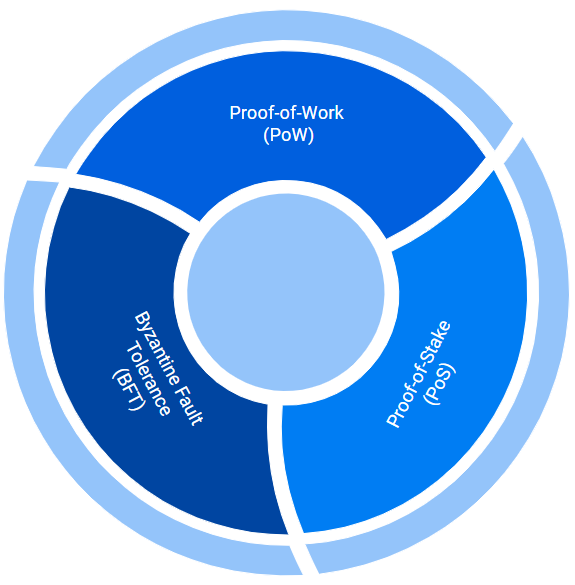
\includegraphics[width=0.6\textwidth]{imagens/algoritmos-consenso.png}
	\caption{Os três algoritmos de consenso mais conhecidos}
\end{figure}


\section{Hyperledger}
Hyperledger\cite{hyperledger} é uma comunidade de código aberto "estabelecida sob a Linux Foundation\cite{linuxfoundation}, que tem uma história longa e muito bem-sucedida de nutrir projetos de código aberto sob uma governança aberta que desenvolve comunidades sustentáveis e ecossistemas prósperos" focada no desenvolvimento de um conjunto de estruturas, ferramentas e bibliotecas para implantação de blockchain em nível corporativo.

\subsection{Hyperledger Fabric}
Hyperledger Fabric\cite{hyperledgerfabric} é uma plataforma do tipo DLT (Distributed Ledger Technologies) de código aberto de nível empresarial, projetada para uso corporativo desde o início.
\begin{figure}[H]
	\centering
	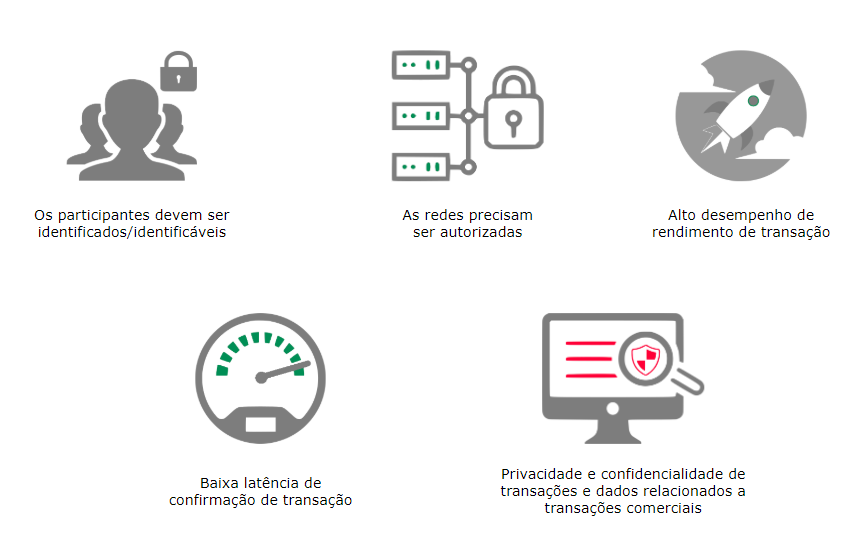
\includegraphics[width=0.9\textwidth]{imagens/requisitos.png}
	\caption{Principais requisitos para uso corporativo}
\end{figure}

\subsection{Criando sua primeira rede Blockchain}
Depois de contextualizarmos sobre o universo Blockchain é chega a hora de partimos para prática.

\begin{lstlisting}[language=bash]
# Oba!! Prática!! 
$ echo "Vamos nessa!"
\end{lstlisting}

A topologia de nossa rede ficará assim:
\begin{figure}[H]
	\centering
	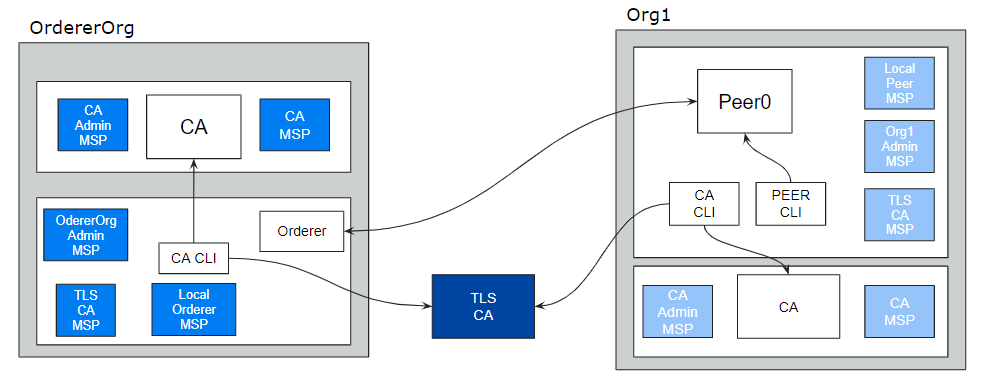
\includegraphics[width=0.7\textwidth]{imagens/primeira-rede.png}
	\caption{Topologia da nossa primeira rede}
\end{figure}

\subsubsection{Pré-requisitos}
Para facilitar, disponibilizei os comandos necessários para configurar o ambiente de desenvolvimento no meu GitHub\cite{configuracaodeambiente}, mas recomendo fortemente que acesse pré-requisitos\cite{prerequisitos} para se familiarizar com os requisitos básicos para rodar uma rede Hyperledger Fabric.

\begin{lstlisting}
  Notas: Este post baseia-se em ambiente Linux (Ubuntu 18.04).
\end{lstlisting}

\subsubsection{Definindo diretório de trabalho}
Vale lembra que os diretórios utilizados para armazenar os binários e arquivos de configuração da rede a seguir não é uma imposição, você pode definir outros caminhos caso deseje, porém será necessário alterar os comandos aqui demonstrados.

\begin{lstlisting}
$ sudo mkdir -p /opt/blockchain/hyperledger/
$ sudo chown -R aluno:aluno /opt/blockchain

# Certifique que esteja no diretório correto
$ cd /opt/blockchain/hyperledger/
\end{lstlisting}

\subsubsection{Baixando Imagens Hyperledger Fabric}
Vamos usar os comandos abaixo para baixar as imagens docker\cite{docker} e os binários necessários para criar a cadeia de certificados e os demais artefatos necessários para configurar a rede Hyperledger\cite{hyperledger} Fabric\cite{hyperledgerfabric}.

\begin{lstlisting}
$ curl -sSL http://bit.ly/2ysbOFE | bash -s 1.4.0

# Após conclusão será criado diretório fabric-samples
$ tree -L 2
\end{lstlisting}
\begin{figure}[H]
	\centering
	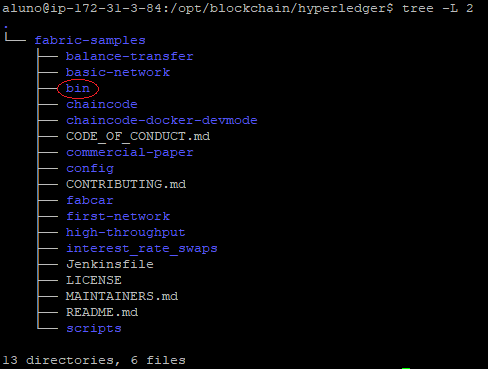
\includegraphics[width=0.7\textwidth]{imagens/path-fabric-samples.png}
	\caption{Estrutura do diretório fabric-samples}
\end{figure}

\subsubsection{Entendendo os binários Fabric\cite{hyperledgerfabric}}
Agora vamos enteder um pouco dos binários Fabric\cite{hyperledgerfabric} enquanto fazemos a geração dos artefatos para nossa rede.

\begin{lstlisting}
# Clonando arquivos de configuracoes
$ git clone -b feature/lab-1 https://github.com/deusimarferreira/hyperledger-fabric.git network

# Acessando diretório dos arquivos
$ cd network

# Variáveis de ambiente
$ export PATH=$GOPATH/src/github.com/hyperledger/fabric/build/bin:${PWD}/../fabric-samples/bin:${PWD}:$PATH
$ export FABRIC_CFG_PATH=${PWD}
$ export CHANNEL_NAME=villalabs-channel
\end{lstlisting}

O primeiro binário que iremos usar será o \textit{cryptogen}, ele é responsável por gerar a cadeia de certificados Hyperledger\cite{hyperledger} Fabrica\cite{hyperledgerfabric} CA (Certificate Authority). Esse binário depende das configurações contidas no arquivo \textit{crypto-config.yaml} e, após execução gera os artefatos no diretório \textit{crypto-config}.
\begin{lstlisting}
# Crie os diretórios crypto-config e channel-artifacts  
$ mkdir crypto-config channel-artifacts

# Agora vamos gerar a cadeia de certificados para CA
$ cryptogen generate --config=./crypto-config.yaml
\end{lstlisting}

O segundo binário que iremos usar será o \textit{configtxgen}, ele é responsável por gerar os artefatos de pré-configuração da rede Hyperledger\cite{hyperledger} Fabrica\cite{hyperledgerfabric}. Esse binário depende das configurações contidas no arquivo \textit{configtx.yaml} e, após execução gerar os artefatos de configuração do canal no diretório \textit{channel-artifacts}.
\begin{lstlisting}
# Gera o bloco genesis
$ configtxgen -profile OrgsOrdererGenesis -outputBlock ./channel-artifacts/genesis.block

#
$ configtxgen -profile OrgsChannel -outputCreateChannelTx ./channel-artifacts/channel.tx -channelID $CHANNEL_NAME

#
$ configtxgen -profile OrgsChannel -outputAnchorPeersUpdate ./channel-artifacts/Org1MSPanchors.tx -channelID $CHANNEL_NAME -asOrg Org1MSP
\end{lstlisting}

\subsubsection{Iniciando nossa rede com docker-compose}
Agora estamos perto de finalizar a criação de nossa rede, mas antes de executar o \textit{docker-compose} precisamos atualizar a variável de ambiente FABRIC\_CA\_SERVER\_CA\_KEYFILE para a nova chave criada quando executamos o comanto \textit{cryptogen generate --config=./crypto-config.yaml}.

\begin{lstlisting}
# Comando para identificar a chave
$ ls -la crypto-config/peerOrganizations/org1.villalabs.co/ca/
\end{lstlisting}
\begin{figure}[H]
  \centering
  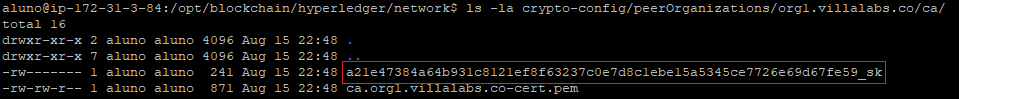
\includegraphics[width=1.1\textwidth]{imagens/env-key.png}
  \caption{Saída do comando ls -la}
\end{figure}

\begin{lstlisting}
# Comando para alterar o docker-compose e incluir a chave 
$ vim docker-compose.yaml
\end{lstlisting}
\begin{figure}[H]
  \centering
  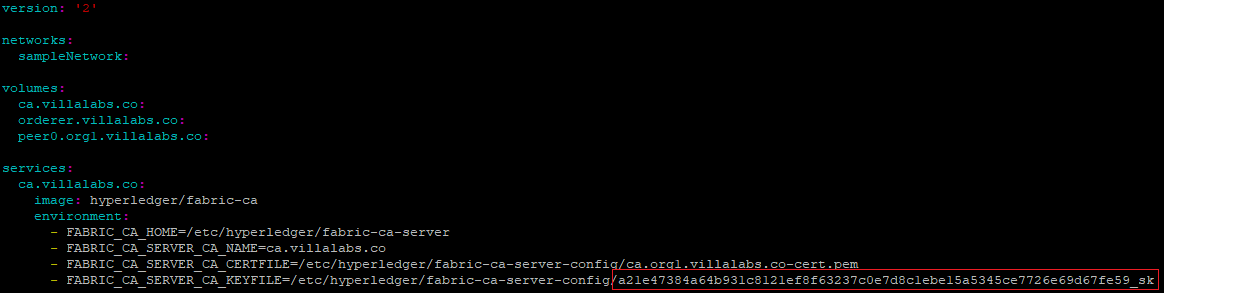
\includegraphics[width=1.1\textwidth]{imagens/env-key-compose.png}
  \caption{docker-compose.yaml}
\end{figure}

\begin{lstlisting}
# Para e limpa todos os containers existentes
$ docker-compose -f docker-compose.yaml down

# Sobre containers
$ docker-compose -f docker-compose.yaml up -d
\end{lstlisting}

Pronto! Após executar o docker-compose, em caso de sucesso veremos o seguinte resultado.
\begin{lstlisting}
# Execute esse comando para verificar os contêineres criados
$ docker ps --format "table {{.ID}}\t{{.Image}}\t{{.Names}}\t{{.Status}}\t{{.Ports}}"
\end{lstlisting}
\begin{figure}[H]
  \centering
  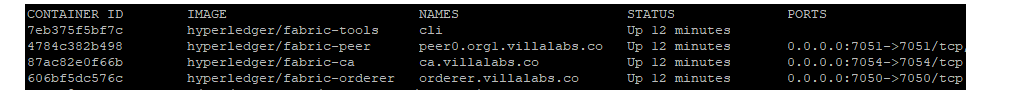
\includegraphics[width=1.1\textwidth]{imagens/conteineres.png}
  \caption{Contêineres criados}
\end{figure}

\subsubsection{Criando canal (channel)}
O teceiro binário tratado até aqui é \textit{peer}, ele é utilizado para administrar o parceiro/par (peer), como cria um canal (channel), implantar um chaincode e etc..

\begin{lstlisting}
# Cria o canal (channel)
$ docker exec \
    -e "CORE_PEER_LOCALMSPID=Org1MSP" \
    -e "CORE_PEER_MSPCONFIGPATH=/etc/hyperledger/msp/users/Admin@org1.villalabs.co/msp" peer0.org1.villalabs.co \
    peer channel create -o orderer.villalabs.co:7050 -c $CHANNEL_NAME -f /etc/hyperledger/configtx/channel.tx
\end{lstlisting}

Saída do comando:
\begin{figure}[H]
  \centering
  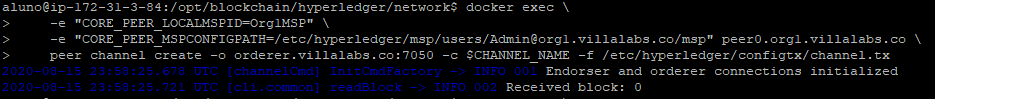
\includegraphics[width=1.1\textwidth]{imagens/criando-canal.png}
  \caption{Canal criado}
\end{figure}

\begin{lstlisting}
# Uni o novo canal (channel) criado
$ docker exec \
    -e "CORE_PEER_LOCALMSPID=Org1MSP" \
    -e "CORE_PEER_MSPCONFIGPATH=/etc/hyperledger/msp/users/Admin@org1.villalabs.co/msp" peer0.org1.villalabs.co \
    peer channel join -b $CHANNEL_NAME.block
\end{lstlisting}

Saída do comando:
\begin{figure}[H]
  \centering
  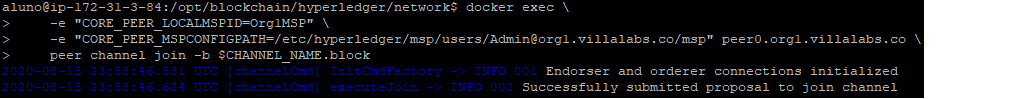
\includegraphics[width=1.1\textwidth]{imagens/join-canal.png}
  \caption{Unindo canal}
\end{figure}

Que tal usar o comando \textit{peer channel list} para verificar o canal recém criado.
\begin{lstlisting}
# Verificar o canal criado
$ docker exec \
    -e "CORE_PEER_LOCALMSPID=Org1MSP" \
    -e "CORE_PEER_MSPCONFIGPATH=/etc/hyperledger/msp/users/Admin@org1.villalabs.co/msp" peer0.org1.villalabs.co \
    peer channel list
\end{lstlisting}

Saída do comando:
\begin{figure}[H]
  \centering
  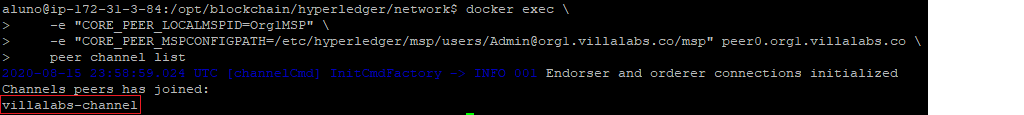
\includegraphics[width=1.1\textwidth]{imagens/lista-canal.png}
  \caption{Canal criado}
\end{figure}

\subsection{Vamos adicionar um novo \textit{peer}}
Até aqui construímos uma rede simples com apenas uma oranização e um peer, mas quando falamos em rede distribuída pensamos em algo maior com várias organizações e peer's. O que tenho a dizer por enquanto é ``muita hora nessa calma, rss'', chegaremos lá.

Nosso próximo passo será adicionar um novo \textit{peer} em nossa \textit{Org1}.

Altere o arquivo \textit{docker-compose.yaml} para adicionar as configurações necessárias para criar o contêiner para o novo \texttt{peer}.

Serão duas alterações necessárias, a primeira nas definições de \textbf{volumes:} e a segunda nos \textbf{services:}.

\textbf{volumes:} - Em volumes adicione o volume para o peer1 (peer1.org1.villalabs.co):
\begin{lstlisting}
volumes:
  ca.villalabs.co:
  orderer.villalabs.co:
  peer0.org1.villalabs.co:
  peer1.org1.villalabs.co:
\end{lstlisting}

\textbf{services:} - Nos services vamos adicionar as configuração abaixo do \textbf{peer0.org1.villalabs.co}:
\begin{lstlisting}
  peer1.org1.villalabs.co:
    container_name: peer1.org1.villalabs.co
    image: hyperledger/fabric-peer
    environment:
      - CORE_VM_ENDPOINT=unix:///host/var/run/docker.sock
      - CORE_PEER_ID=peer1.org1.villalabs.co
      - CORE_LOGGING_PEER=info
      - CORE_CHAINCODE_LOGGING=debug
      - CORE_PEER_LOCALMSPID=Org1MSP
      - CORE_PEER_MSPCONFIGPATH=/etc/hyperledger/msp/peer/
      - CORE_PEER_ADDRESS=peer1.org1.villalabs.co:7051
      - CORE_VM_DOCKER_HOSTCONFIG_NETWORKMODE=network_sampleNetwork
    working_dir: /opt/gopath/src/github.com/hyperledger/fabric
    command: peer node start
    ports:
      - 8051:7051
      - 8053:7053
    volumes:
      - /var/run/:/host/var/run/
      - ./crypto-config/peerOrganizations/org1.villalabs.co/peers/peer1.org1.villalabs.co/msp:/etc/hyperledger/msp/peer
      - ./crypto-config/peerOrganizations/org1.villalabs.co/users:/etc/hyperledger/msp/users
      - ./channel-artifacts:/etc/hyperledger/configtx
    depends_on:
      - orderer.villalabs.co
    networks:
      - sampleNetwork
\end{lstlisting}

Altere também o arquivo \textit{crypto-config.yaml} para aumentar o números de \textit{peer's}.
\begin{lstlisting}
  Template:
    Count: 2
\end{lstlisting}

Usando o binário \textit{cryptogen} para extender nossa rede e adicionar o novo peer.
\begin{lstlisting}
# Realiza a geração da cadeia de certificados para o novo peer
$ cryptogen extend --config=./crypto-config.yaml

# Verifique novo peer adicionado
$ ls -l ./crypto-config/peerOrganizations/org1.villalabs.co/peers/
\end{lstlisting}

Saída do comando:
\begin{figure}[H]
  \centering
  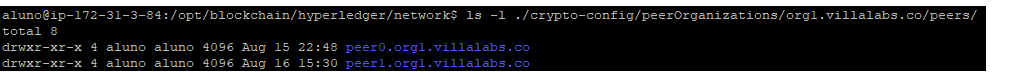
\includegraphics[width=1.1\textwidth]{imagens/output-cryptogen-extend.png}
  \caption{Peer's existentes}
\end{figure}

Usando o binário \textit{configtxgen} para atualizar nossa rede e permitir adicionar o \textit{peer1}.
\begin{lstlisting}
# Vamos gerar nosso genesis block
$ configtxgen -profile OrgsOrdererGenesis -outputBlock ./channel-artifacts/genesis.block
\end{lstlisting}

Tudo pronto, vamos iniciar os contêineres:
\begin{lstlisting}
# Vamos iniciar os containers
$ docker-compose -f docker-compose.yaml up \
  -d peer0.org1.villalabs.co peer1.org1.villalabs.co cli

# Visualize os contêineres com filtro ``name=peer``
$ docker ps --filter name=peer --format "table {{.ID}}\t{{.Image}}\t{{.Names}}\t{{.Status}}\t{{.Ports}}"
\end{lstlisting}

Saída do comando:
\begin{figure}[H]
  \centering
  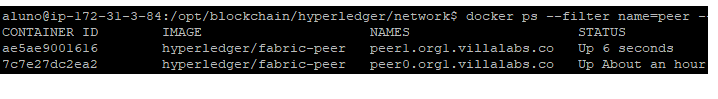
\includegraphics[width=1.1\textwidth]{imagens/conteineres-2.png}
  \caption{Contêineres peer's}
\end{figure}

Agora vamos unir o canal criado no item \textbf{2.2 Criando sua primeira rede Blockchain} ao novo \textit{peer} que acabamos de adicionar.
\begin{lstlisting}
# Primeiro vamos fazer um fetch do genesis block para o corrente channel
$ docker exec \
    -e "CORE_PEER_LOCALMSPID=Org1MSP" \
    -e "CORE_PEER_MSPCONFIGPATH=/etc/hyperledger/msp/users/Admin@org1.villalabs.co/msp" peer1.org1.villalabs.co \
    peer channel fetch oldest $CHANNEL_NAME.block -c $CHANNEL_NAME \
    --orderer orderer.villalabs.co:7050
\end{lstlisting}

Saída do comando:
\begin{figure}[H]
  \centering
  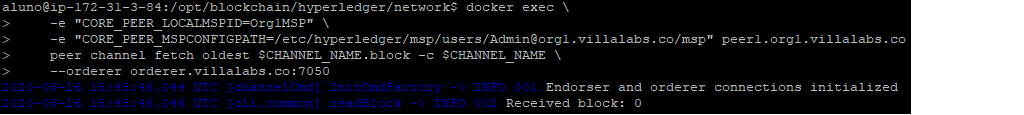
\includegraphics[width=1.1\textwidth]{imagens/output-org1-peer1-fetch.png}
  \caption{Saída do comando peer channel fetch}
\end{figure}

\begin{lstlisting}
# Segundo, vamos executar um join
$ docker exec \
    -e "CORE_PEER_LOCALMSPID=Org1MSP" \
    -e "CORE_PEER_MSPCONFIGPATH=/etc/hyperledger/msp/users/Admin@org1.villalabs.co/msp" peer1.org1.villalabs.co \
    peer channel join -b $CHANNEL_NAME.block
\end{lstlisting}

Saída do comando:
\begin{figure}[H]
  \centering
  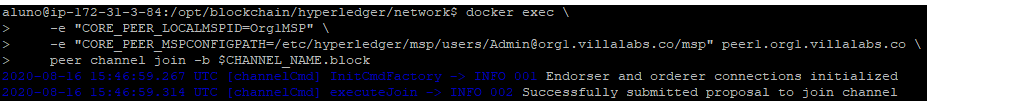
\includegraphics[width=1.1\textwidth]{imagens/output-org1-peer1-join.png}
  \caption{Saída do comando peer channel join}
\end{figure}

Que tal usar o comando \textit{peer channel list} para verificar o canal recém criado.
\begin{lstlisting}
# Verificar o canal
$ docker exec \
    -e "CORE_PEER_LOCALMSPID=Org1MSP" \
    -e "CORE_PEER_MSPCONFIGPATH=/etc/hyperledger/msp/users/Admin@org1.villalabs.co/msp" peer1.org1.villalabs.co \
    peer channel list
\end{lstlisting}

Saída do comando:
\begin{figure}[H]
  \centering
  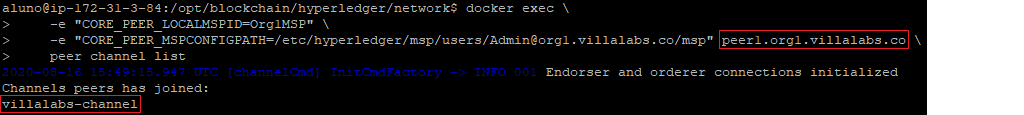
\includegraphics[width=1.1\textwidth]{imagens/output-org1-peer1-list.png}
  \caption{Saída do comando peer channel list}
\end{figure}

\subsection{Usando CouchDB como banco de estado}
Por padrão o Hyperledger\cite{hyperledger} Fabric\cite{hyperledgerfabric} usa como banco de dados de estado o LevelDB, nesta seção iremos apresentar como configurar o CouchDB como nosso banco de dados de estado nos \texttt{peer's} de nossa rede.

Todo \textit{peer} na rede deve possuir uma cópia do \textit{ledger} e um \textit{state database} própio. Novamente vamos alterar o arquivo \textit{docker-compose.yaml} (O arquivo completo pode ser encontrado no endereço https://github.com/deusimarferreira/hyperledger-fabric/blob/feature/lab-3/docker-compose.yaml) para alterar e incluir as configurações necessárias.

Adicione as variáveis de ambiente nas configurações dos \textit{peer's} (\textit{peer0} e \textit{peer1}).
\begin{lstlisting}
# Peer0
CORE_LEDGER_STATE_STATEDATABASE=CouchDB
CORE_LEDGER_STATE_COUCHDBCONFIG_COUCHDBADDRESS=couchdb.peer0.org1.villalabs.co:5984
CORE_LEDGER_STATE_COUCHDBCONFIG_USERNAME=peer0.org1
CORE_LEDGER_STATE_COUCHDBCONFIG_PASSWORD=password

# Peer1
CORE_LEDGER_STATE_STATEDATABASE=CouchDB
CORE_LEDGER_STATE_COUCHDBCONFIG_COUCHDBADDRESS=couchdb.peer1.org1.villalabs.co:5984
CORE_LEDGER_STATE_COUCHDBCONFIG_USERNAME=peer1.org1
CORE_LEDGER_STATE_COUCHDBCONFIG_PASSWORD=password
\end{lstlisting}

\textbf{services:} - Nos services vamos adicionar as configuração dos dois bancos de estado:
\begin{lstlisting}
  couchdb.peer0.org1.villalabs.co:
    container_name: couchdb.peer0.org1.villalabs.co
    environment:
      - COUCHDB_USER=peer0.org1
      - COUCHDB_PASSWORD=password
    image: hyperledger/fabric-couchdb
    ports: 
      - 5984:5984
    networks: 
      - sampleNetwork

  couchdb.peer1.org1.villalabs.co:
    container_name: couchdb.peer1.org1.villalabs.co
    environment:
      - COUCHDB_USER=peer1.org1
      - COUCHDB_PASSWORD=password
    image: hyperledger/fabric-couchdb
    ports: 
      - 6984:5984
    networks: 
      - sampleNetwork
\end{lstlisting}

Tudo pronto, vamos iniciar os contêineres:
\begin{lstlisting}
$ docker-compose -f docker-compose.yaml up \
  -d ca.villalabs.co orderer.villalabs.co \
  couchdb.peer0.org1.villalabs.co peer0.org1.villalabs.co \
  couchdb.peer1.org1.villalabs.co peer1.org1.villalabs.co \
  cli

# Visualize os contêineres
$ docker ps --format "table {{.ID}}\t{{.Image}}\t{{.Names}}\t{{.Status}}\t{{.Ports}}"
\end{lstlisting}

Saída do comando:
\begin{figure}[H]
  \centering
  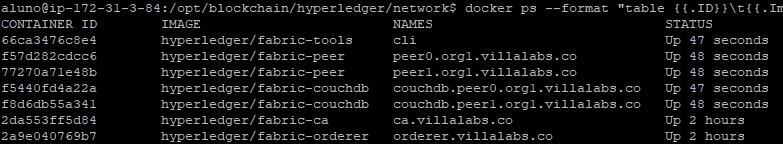
\includegraphics[width=1.1\textwidth]{imagens/conteineres-3.png}
  \caption{Contêineres}
\end{figure}

Use o comando \textit{curl} para testar as bases CouchDB:
\begin{lstlisting}
# Testar CouchBD
$ curl http://localhost:5984
$ curl http://localhost:6984
\end{lstlisting}

Como mudamos de base de dados iremos precisar atualizar os \textit{peer's}:
\begin{lstlisting}
# PEER0
# Primeiro vamos fazer um fetch do genesis block para o corrente channel
$ docker exec \
    -e "CORE_PEER_LOCALMSPID=Org1MSP" \
    -e "CORE_PEER_MSPCONFIGPATH=/etc/hyperledger/msp/users/Admin@org1.villalabs.co/msp" peer0.org1.villalabs.co \
    peer channel fetch oldest $CHANNEL_NAME.block -c $CHANNEL_NAME \
    --orderer orderer.villalabs.co:7050

# Segundo, vamos executar um join
$ docker exec \
    -e "CORE_PEER_LOCALMSPID=Org1MSP" \
    -e "CORE_PEER_MSPCONFIGPATH=/etc/hyperledger/msp/users/Admin@org1.villalabs.co/msp" peer0.org1.villalabs.co \
    peer channel join -b $CHANNEL_NAME.block

# PEER1
# Primeiro vamos fazer um fetch do genesis block para o corrente channel
$ docker exec \
    -e "CORE_PEER_LOCALMSPID=Org1MSP" \
    -e "CORE_PEER_MSPCONFIGPATH=/etc/hyperledger/msp/users/Admin@org1.villalabs.co/msp" peer1.org1.villalabs.co \
    peer channel fetch oldest $CHANNEL_NAME.block -c $CHANNEL_NAME \
    --orderer orderer.villalabs.co:7050

# Segundo, vamos executar um join
$ docker exec \
    -e "CORE_PEER_LOCALMSPID=Org1MSP" \
    -e "CORE_PEER_MSPCONFIGPATH=/etc/hyperledger/msp/users/Admin@org1.villalabs.co/msp" peer1.org1.villalabs.co \
    peer channel join -b $CHANNEL_NAME.block
\end{lstlisting}

Que tal usar o comando \textit{peer channel list} para verificar o canal recém criado.
\begin{lstlisting}
# PEER0
# Verificar o canal
$ docker exec \
    -e "CORE_PEER_LOCALMSPID=Org1MSP" \
    -e "CORE_PEER_MSPCONFIGPATH=/etc/hyperledger/msp/users/Admin@org1.villalabs.co/msp" peer0.org1.villalabs.co \
    peer channel list

# PEER1
# Verificar o canal
$ docker exec \
    -e "CORE_PEER_LOCALMSPID=Org1MSP" \
    -e "CORE_PEER_MSPCONFIGPATH=/etc/hyperledger/msp/users/Admin@org1.villalabs.co/msp" peer1.org1.villalabs.co \
    peer channel list
\end{lstlisting}

\section{Conclusão}
Ne artigo tivemos a oportunidade de conhecer um pouco mais sobre a tecnologia Blockchain e ainda criar uma rede na prática usando a ferramenta Hyperledger\cite{hyperledger} Fabric\cite{hyperledgerfabric}. 

\section{Sobre o autor}
Praticante dos princípios ágeis para desenvolvimento de software, focado na entrega de valor.

Adepto do software \textbf{Open Source} (Software Livre), estou sempre em busca de novos conhecimentos e desafios relacionados ao desenvolvimento de software que agregam valor tanto no âmbito pessoal quanto profissional. 

\begin{center}
``\underline{Livre} significa que esta apostila é gratuita e pode ser compartilhada a vontade. \underline{Open Source} além de livre todos os arquivos que permitem a geração desta (chamados de arquivos fontes) devem ser disponibilizados para que qualquer pessoa possa modificar ao seu prazer, gerar novas, complementar ou fazer o que quiser.''
por Fernando Anselmo\cite{fernandoanselmo}
\end{center}

%--------------------------------------------------------------------------
% REFERÊNCIAS
%--------------------------------------------------------------------------
\begin{thebibliography}{5}
  \bibitem{linuxfoundation} 
  The Linux Foundation \\
  \url{https://www.linuxfoundation.org/}

  \bibitem{hyperledger} 
  Hyperledger \\
  \url{https://hyperledger.org/}

  \bibitem{hyperledgerfabric} 
  Hyperledger Fabric \\
  \url{https://www.hyperledger.org/use/fabric}

  \bibitem{staurthaber}
  Staurt Haber
  \url(https://www.linkedin.com/in/stuart-haber/)

  \bibitem{scottstornetta}
  W. Scott Stornetta \\
  \url(https://www.linkedin.com/in/w-scott-stornetta-25186120/)

  \bibitem{criadoresblockchain}
  How to Time-Stamp a Digital Document \\
  \url{https://link.springer.com/chapter/10.1007%2F3-540-38424-3_32}

  \bibitem{bitcoin}
  Bitcoin White paper \\
  \url{https://bitcoin.org/en/bitcoin-paper}

  \bibitem{configuracaodeambiente}
  Configurações de Ambiente \\
  \url{https://github.com/deusimarferreira/hyperledger-fabric/blob/master/environment.md}
  \url{https://bitcoin.org/en/bitcoin-paper}

  \bibitem{prerequisitos}
  Pré-requisitos \\
  \url{https://hyperledger-fabric.readthedocs.io/en/release-1.4/prereqs.html}
  
  \bibitem{docker}
  Docker \\
  \url{https://www.docker.com/}

  	\bibitem{latex} 
	LaTeX \\
	\url{https://latex.net/}
	
	\bibitem{credito} 
	Essa apostila utiliza scripts LaTeX\cite{latex} disponibilizados por Fernando Anselmo\cite{fernandoanselmo}  \\
	\url{https://github.com/fernandoans/publicacoes}

	\bibitem{fernandoanselmo} 
	Fernando Anselmo - Blog Oficial de Tecnologia \\
	\url{http://www.fernandoanselmo.blogspot.com.br/}

	\bibitem{publicacaofernando}
	Encontre publicações de Fernando Anselmo\cite{fernandoanselmo} em \\
	\url{https://cetrex.academia.edu/FernandoAnselmo}

	\bibitem{github} 
	Encontre essa e outras publicações minhas em \\
	\url{https://github.com/deusimarferreira/artigos}
\end{thebibliography}
  
\end{document}
